\documentclass[tikz, crop, border = {2pt 2pt 2pt 2pt}]{standalone}

\usepackage{concmath-otf}
\usetikzlibrary{calc, angles, quotes, patterns}
\usetikzlibrary{decorations.pathreplacing, decorations.pathmorphing, calligraphy}
\usetikzlibrary{math}

\begin{document}
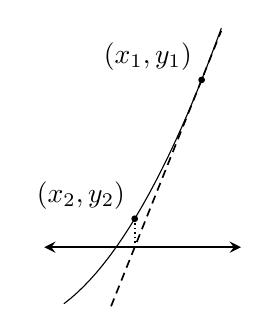
\begin{tikzpicture}
	\draw[domain = 0.75:2.75] plot (\x, {1/2*\x*\x - 1});
	\draw[stealth-stealth, thick] (0.5, 0) -- (3, 0);
	
	\tikzmath{
		function f(\x) {
			return 1/2*\x*\x - 1;
		};
		\fp = 2.5;
		\yfp = f(\fp);
	}
	\filldraw (\fp, \yfp) circle (1pt) node[above left]{$(x_1, y_1)$};
	\draw[densely dashed, semithick, domain = 1.35:2.75, smooth] plot (\x, {\fp*(\x - \fp) + \yfp});
	\draw[densely dotted, semithick] ({-\yfp/\fp + \fp}, 0) -- ++ (0, {f(-\yfp/\fp + \fp)});
	\filldraw ({-\yfp/\fp + \fp}, {f(-\yfp/\fp + \fp)}) circle (1pt) node[above left]{$(x_2, y_2)$};
\end{tikzpicture}
\end{document}
